\documentclass[80pt]{article}
\usepackage{arxiv}

\usepackage[utf8]{inputenc}
\usepackage[english]{babel}
\usepackage[T1]{fontenc}
\usepackage{url}
\usepackage{booktabs}
\usepackage{amsfonts}
\usepackage{amsmath}
\usepackage{nicefrac}
\usepackage{microtype}
\usepackage{lipsum}
\usepackage{graphicx}
\usepackage{natbib}
\usepackage{doi}
\usepackage{subfig, epsfig}

\graphicspath{ {../figures/} }

\title{Anti-Distillation: Knowledge Transfer from Simple Model to a Complex One}

\author{\textbf{Kseniia~Petrushina,~Andrey~Grabovoy,~Oleg Bakhteev,~Vadim~Strijov} \\
	Moscow Institute of Physics and Technology \\
	\texttt{\{petrushina.ke,~grabovoy.av,~bakhteev,~strijov\}@phystech.edu}
}
\date{}
\renewcommand{\undertitle}{}
\renewcommand{\headeright}{}
\renewcommand{\shorttitle}{Anti-Distillation: Knowledge Transfer from Simple Model to a Complex One}

\hypersetup{
pdftitle={Anti-Distillation: Knowledge Transfer from Simple Model to a Complex One},
pdfauthor={Kseniia~Petrushina},
pdfkeywords={Distillation, Knowledge Transfer, Weight Initialization, Machine Learning},
}

\begin{document}
\maketitle

\begin{abstract}
	This paper considers the problem of adapting the model to new data with a large amount of information. We propose to build a more complex model using the parameters of a simple one. It is necessary to take into account not only the accuracy of the prediction on the original samples but also the adaptability to new data and the stability of the obtained solution. The novelty of the work lies in the fact that our method allows adapting the pre-trained model to a more heterogeneous dataset. This study uses both probabilistic and algebraic methods for obtaining a student model. In the computational experiment, we analyse the quality of predictions on Fashion-Mnist and CIFAR10 datasets.
\end{abstract}

\keywords{Distillation \and Knowledge Transfer \and Weight Initialization \and Machine Learning}

\section{Introduction}
Training a model from scratch can lead to poor results or take a long time. To get better results faster, researchers have been developing various methods allowing to use existing trained models to solve new problems. For instance, there are knowledge distillation \citep{hinton2015distilling, lopezpaz2016unifying}, transfer learning \citep{zhuang2019acomprehensive}, fine-tuning, low-rank model approximation \citep{yu2017oncompressing}. Moreover, there are methods for initializing model weights for faster convergence \citep{glorot2010understanding}. These approaches help to decrease the time needed for training or inference and achieve higher quality.

Consider the distillation method. Statement of the initial problem is the transfer of knowledge from a cumbersome neural network or ensemble of ones to a smaller model in the classification problem. Hinton and others \citep{hinton2015distilling} were able to achieve this by training the student model to reproduce the probability distribution of the classes produced by the teacher model. The use of such soft targets helped to carry more information, so the student models generalization ability is comparable to the teachers. However, this research focuses on reducing model parameters under conditions of input data persistence. We want to solve the inverse problem: to keep the model properties under conditions of increasing sample complexity.

This work proposes a method for increasing the complexity of the model based on a pre-trained one. This is done by growing the dimension of the weight space and initializing part of the student neural network with teacher model weights. Our approach allows to speed up neural network training and obtain a more robust model. In this way, we can adapt the pre-trained model to more variable data and reuse previously learned information.

This paper presents computational experiments on various ways of complicating the model. We consider fully connected, convolutional layers and LSTM modules. The experiment compares uniform initialization with one based on a previously trained model and analyse differences in convergence rate, prediction variance, and achieved quality.

\section{Anti-Distillation problem statement}
Consider $c$-class classification. There are two sets
$$D_1 = \{(\mathbf{x}_i, y_i)\}_{i=1}^{m_1},~\mathbf{x}_i \in \mathbb{R}^{n_1},~y_i \in C_1 = \{1, \dots, c_1\},$$

$$D_2 =  \{(\mathbf{x}'_i, y'_i)\}_{i=1}^{m_2},~\mathbf{x}'_i \in \mathbb{R}^{n_2},~y'_i \in C_2 = \{1, \dots, c_2\}.$$

Set $D_2$ is \textit{more complex} than $D_1$, i.e., $n_2 > n_1$ or $c_2 > c_1$.

Having the teacher model 

\[g_\text{tr}: \mathbb{R}^{n_1} \rightarrow \Delta^{c_1},~g_\text{tr}(\mathbf{x}) = g(\mathbf{x}, \hat{\mathbf{u}}),\] 

where optimal model parameters $\hat{\mathbf{u}} \in \mathbb{R}^{N_{\text{tr}}}$ are defined as follows:
$$\hat{\mathbf{u}} =  \underset{\mathbf{u}}{\arg\min}~\mathcal{L}_g(\mathbf{u}, D_1) =\underset{\mathbf{u}}{\arg\min}~\sum\limits_{i=1}^{m_1} l \bigl(y_i,~g(\mathbf{x}_i, \mathbf{u})\bigr),$$
here, $l$ is a cross-entropy loss 
$$l(y, \hat{y}) = -\sum\limits_{k=1}^{c} [y = k] \log{\hat{y}_k},~y \in C,~\hat{y} \in \Delta^c,$$

where $\Delta^c$ is the set of $c$-dimentional probability vectors,

our approach proposes constructing the student model

\[f_\text{st}: \mathbb{R}^{n_2} \rightarrow \Delta^{c_2},~f_\text{st}(\mathbf{x}) = f(\mathbf{x}, \hat{\mathbf{w}}),\]

$$\hat{\mathbf{w}} =  \underset{\mathbf{w}}{\arg\min}~\mathcal{L}_f(\mathbf{w}, D_2).$$

We find the solution to the above optimization problem using gradient optimization methods. The model weights $\mathbf{w} \in \mathbb{R}^{N_{\text{st}}}$ update as
\[\mathbf{w}_{t+1} = T(\mathbf{w}_t |~\mathcal{L}_f,~D_2),\]
\[T: \mathbb{R}^{N_\text{st}} \rightarrow \mathbb{R}^{N_\text{st}}\]

is the optimization operator and $t \in \mathbb{N}$ is the gradient step number.

The function 
\[\varphi: \mathbb{R}^{N_\text{tr}} \rightarrow \mathbb{R}^{N_\text{st}}\]

determines the student model parameters initialization $\mathbf{w}_1 = \varphi(\hat{\mathbf{u}})$.

\section{Our setup}
\label{sec:setup}

We construct a more complex model by extending fully connected layers and increasing number of feature maps in convolutional layers. There are different initialization methods for extended weights:

\begin{enumerate}
    \item Zero initialization.
    \item Uniform initialization $U[0, \theta]$.
\end{enumerate}

\section{Theory}

We define the function $\varphi: \mathbb{R}^{N_\text{tr}} \rightarrow \mathbb{R}^{N_\text{st}}$ as
$$\varphi(\mathbf{u}) = \underset{\mathbf{w}}{\arg\min}~\mathcal{L}(\mathbf{w}),$$
where \[\mathcal{L} = \lambda_1 \mathcal{L}_f(\mathbf{w}, D_1^*) + \lambda_2 \mathcal{L}_2 (\mathbf{w}, \mathbf{u}) + \lambda_3 \mathcal{L}_3^\delta (\mathbf{w}, D_1) + \lambda_4 \mathcal{L}_4 \bigl(\displaystyle \frac{\partial^2 \mathcal{L}_f}{\partial \mathbf{w}^2}\bigr).\]

\begin{enumerate}
    \item $\mathcal{L}_f(\mathbf{w}, D_1^*)$ loss is responsible for having the optimal weights on the $D_1^* = \{(\psi (\textbf{x}), y \;|\; (\textbf{x}, y) \in D_1\}$, $\psi: \mathbb{R}^{n_1} \rightarrow \mathbb{R}^{n_2}$.
    \item $\mathcal{L}_2 (\mathbf{w}, \mathbf{u}) = \|\textbf{u} - \textbf{w}[\textbf{u}]\|^2_2$ provides a small difference between the weights of the teacher model and the student model in the respective places.
    \item $\mathcal{L}_3^\delta (\mathbf{w}, D_1) = \displaystyle \sum \limits_{(\textbf{x}, y) \in D_1} \displaystyle \mathbb{E}_{\textbf{x}' \in U_\delta(\textbf{x})} \mathcal{L}_f(\mathbf{w}, \textbf{x}', y)$  and  $\mathcal{L}_4 \bigl(\displaystyle \frac{\partial^2 \mathcal{L}_f}{\partial \mathbf{w}^2}\bigr) = \|\bigl(\displaystyle \frac{\partial^2 \mathcal{L}_f}{\partial \mathbf{w}^2}\bigr)\|^2_2$ losses account for stability of solution to noise in input data.
\end{enumerate}

Wherein \[\sum\limits_{i=1}^4 \lambda_i =1, \forall\; i \in \overline{1, 4}:\; \lambda_i \ge 0.\]
In case of Anti-Distillation $\lambda_2 >0$. 

Quality criterion is $\mathcal{L}_3^\delta (\mathbf{w}^*, D_2)$, since we are interested in getting a model that is resistant to input data corruption. In addition, we consider accuracy of predictions on $D_2$ set.

\newtheorem{hypothesis}{Hypothesis}
\begin{hypothesis}
Student models initialized by the result of applying the function $\varphi$ to the weights of the pre-trained teacher model are more persistent and achieve higher accuracy than models with default weights.
\end{hypothesis}

\section{Computational experiment}

The goal of computational experiment is to compare the performance of models depending on the initialization of parameters. 

\subsection{Data}

\begin{enumerate}
    \item Fashion-MNIST is a dataset of Zalando's article images consisting of a training set of 60,000 examples and a test set of 10,000 examples. Each example is a 28x28 grayscale image, associated with a label from 10 classes  \citep{fashionmnist}.
    
    \item The CIFAR-10 dataset consists of 60000 32x32 colour images in 10 classes, with 6000 images per class. There are 50000 training images and 10000 test images \citep{cifar10}.
\end{enumerate}

\subsection{Configuration of algorithm run}

We carry out the experiments as follows: we train the teacher model, increase its complexity as described in \autoref{sec:setup}, and compare different ways of initializing the weights of the model. There are three cases under consideration: uniform initialization of all model weights, zero and uniform initialization of extended weights. We compare them by measuring accuracy of predictions, cross-entropy loss value on validation sample, and prediction variance. Also we investigate the case of noisy input data, considering above quality measures depending on the percentage of image corrupted.

\subsection{List of expected tables and figures}

\begin{enumerate}
    \item Graph of accuracy/loss versus epoch number for different ways of initialization on the same dataset (Fashion-MNIST) -- basic experiment \ref{fig:1}.
    \item Graph of accuracy/loss versus image corruption percentage for different ways of initialization on the same dataset.
    \item Table with accuracy/loss depending on the initialization method (in this case we train the teacher model on subset of Fasion-MNIST classes, and the student model on full dataset).
    \item Table with accuracy/loss depending on the initialization method (in this case we train the teacher model on Fasion-MNIST classes, and the student model on CIFAR-10).
\end{enumerate}

\subsection{Preliminary report}

It follows from the result that zero initialization on average outperformes other initialization methods. As seen in \ref{fig:1} uniform initialization of extended weights has the smallest variance, but this method on average worse than others. It is worth paying attention to checking other values of $\theta$, where extended uniform parameters selects from $U[0, \theta]$. As due to large $\theta$ values, information from the teacher model may be lost.

\begin{figure}[!t]
  \subfloat{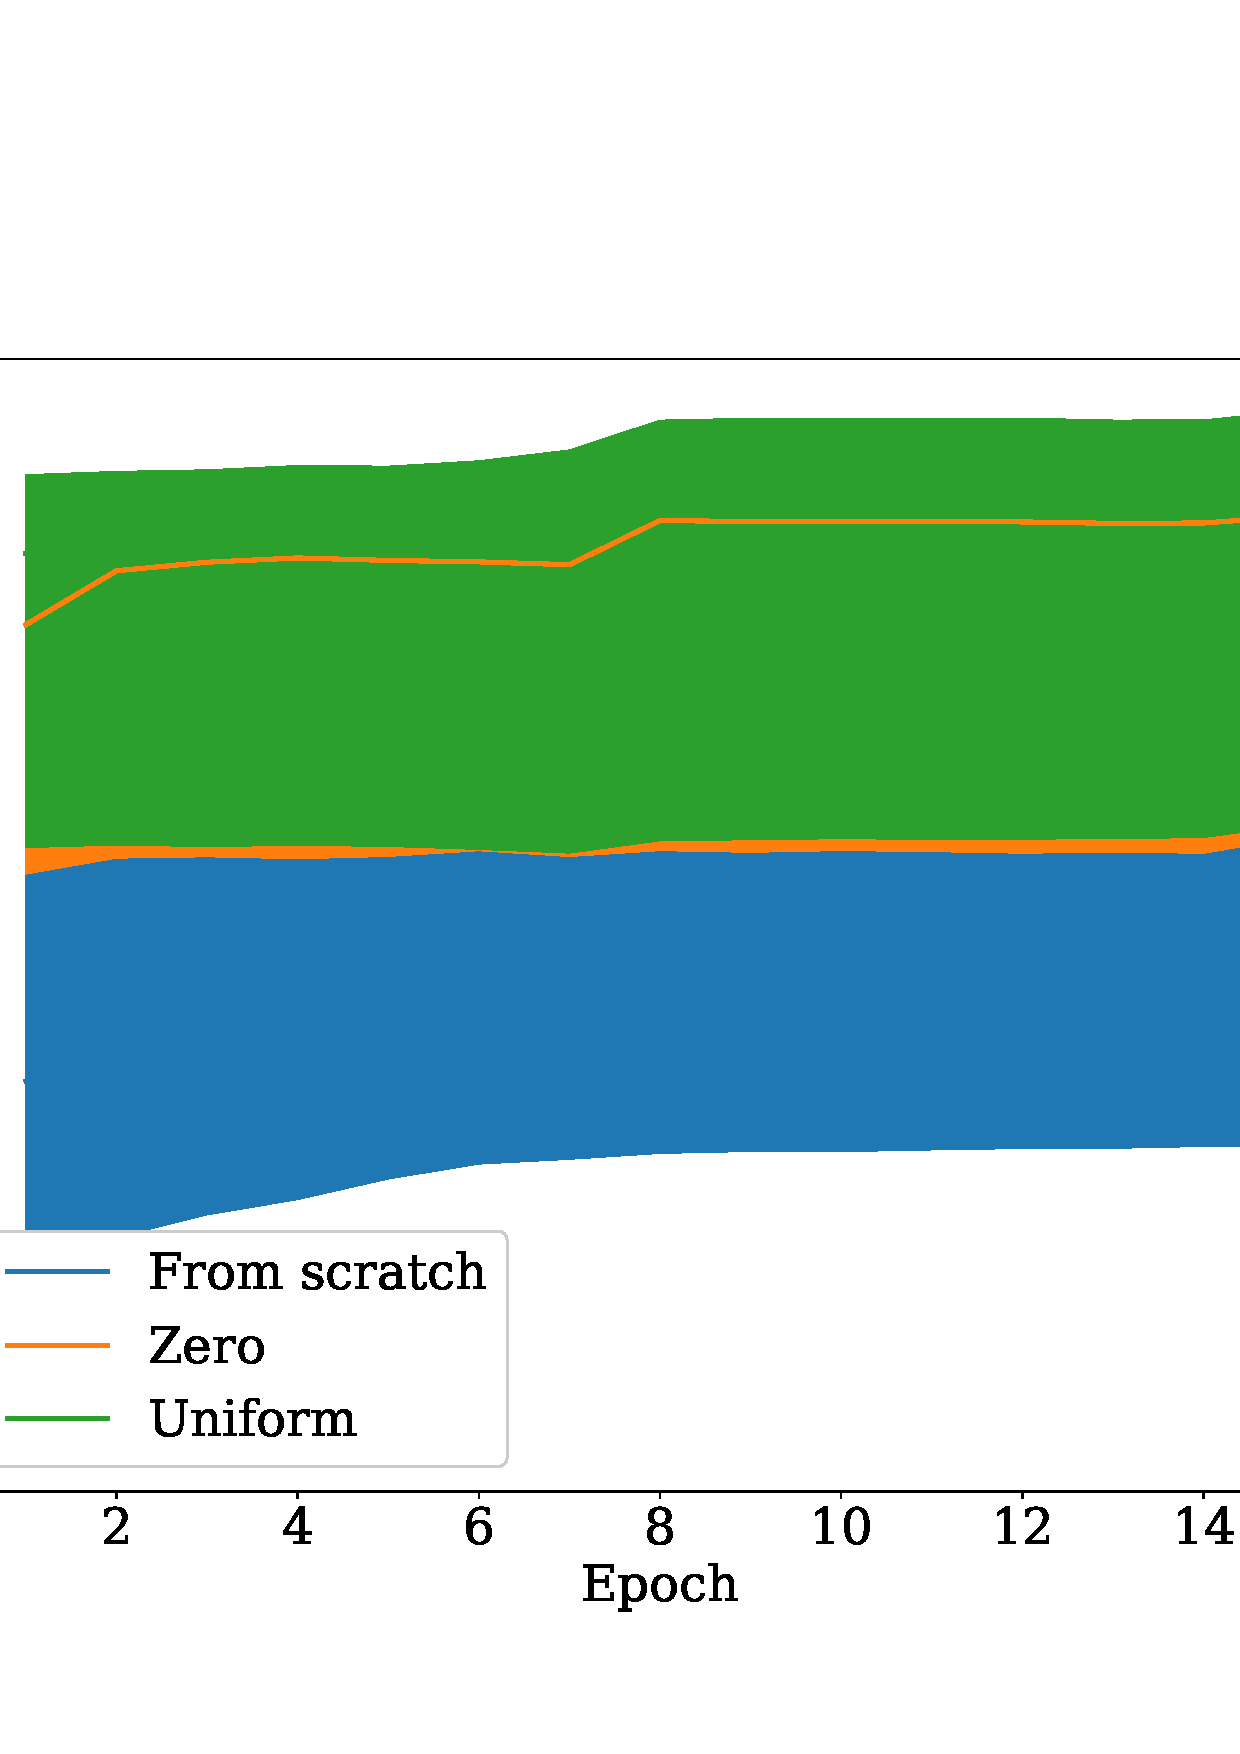
\includegraphics[width=0.5\textwidth]{base_acc.png}}
  \subfloat{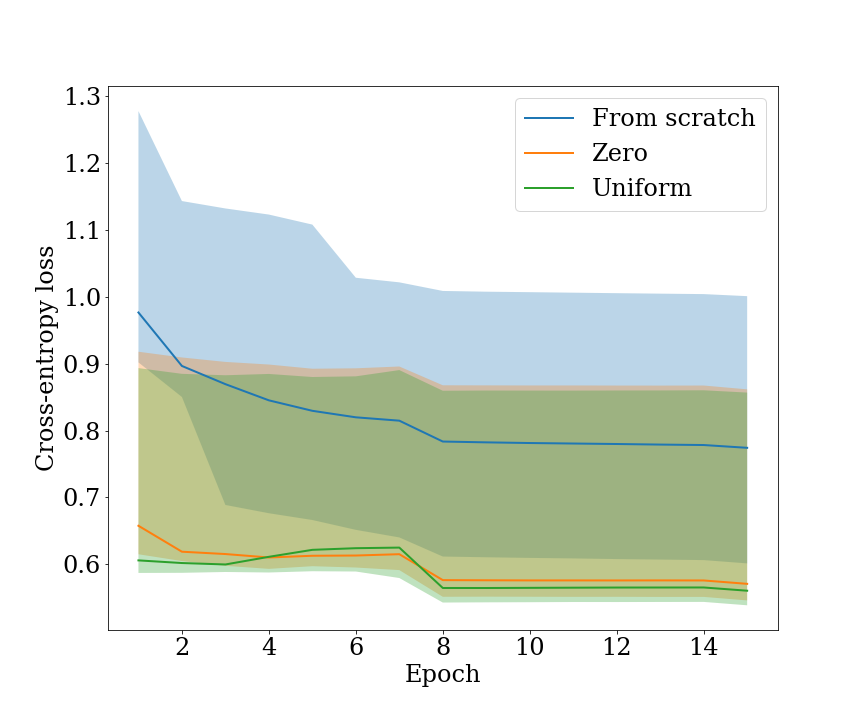
\includegraphics[width=0.5\textwidth]{base_loss.png}}\\
 \caption{Comparison of quality metrics for different initialization methods}
  \label{fig:1}
\end{figure}

\subsection{Error analysis}

For the experiment we compare two ways of initialization: uniform initialization and initialization with $\varphi(\textbf{u}^*)$, where $\lambda_2 = 1$, i.e., preserving the teacher model weights and uniformly initializing extended ones. 

\begin{figure}[!t]
  \subfloat{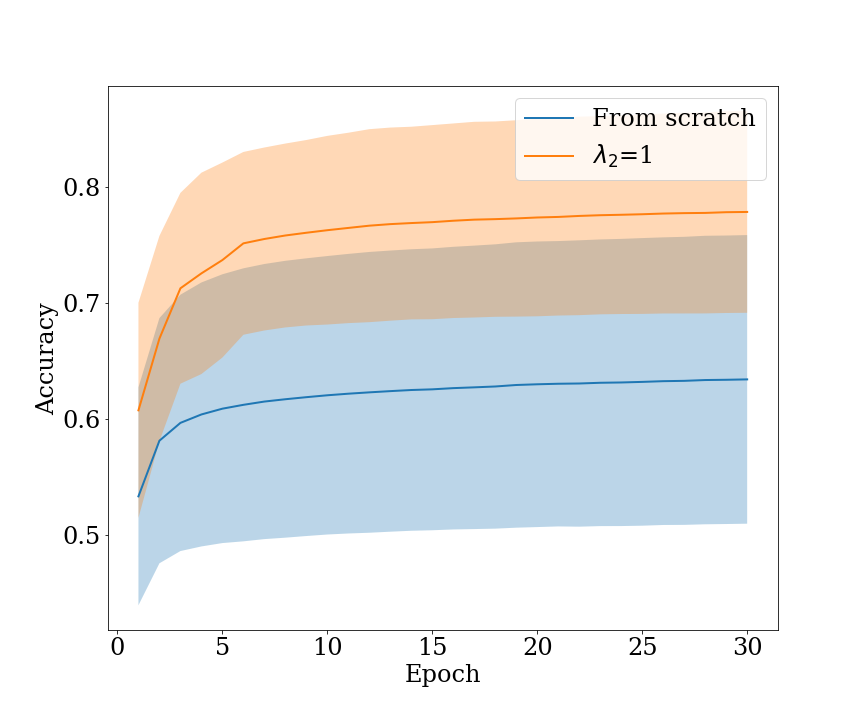
\includegraphics[width=0.5\textwidth]{l2_acc.png}}
  \subfloat{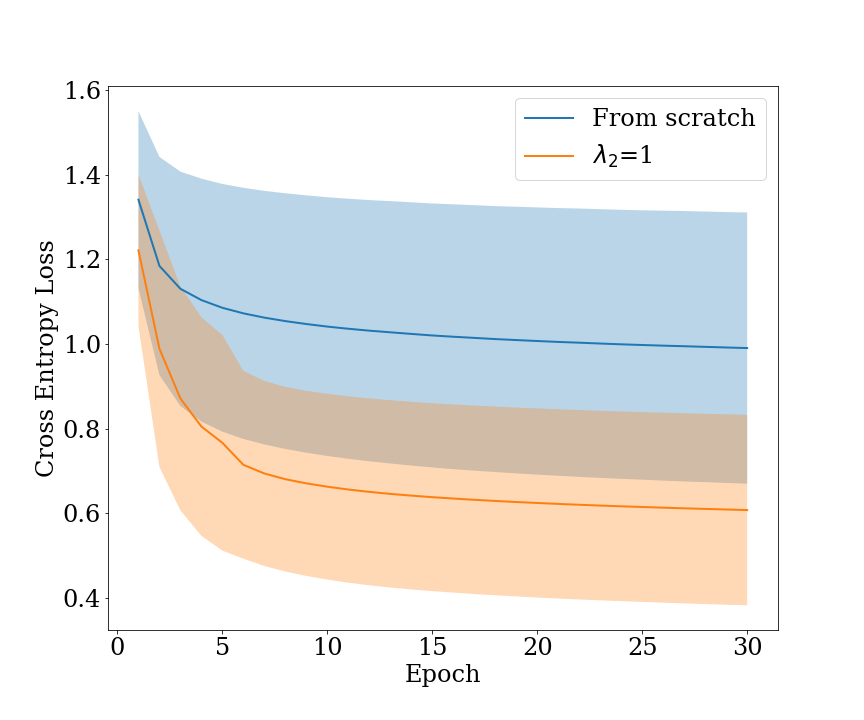
\includegraphics[width=0.5\textwidth]{l2_loss.png}}\\
 \caption{Comparison of quality metrics for different initialization methods}
  \label{fig:2}
\end{figure}

\newpage

\bibliographystyle{plain}
\bibliography{Petrushina2022AntiDistillation.bib}

\end{document}